\section{Demarche Expérimentale}

Le montage expérimental représenté à la figure \ref{fig:montage} permet de mesurer la tension \(U_D\) et l'intensité \(I_R\) à la sortie des différentes technologies de cellules solaires, le Si amorphe (A), Si monocristallin (M) et Si polycristallin (P), en fonction d'une résistance de charge variable \(R_C\).
Toutes les cellules ont une surface \(S = (100 \pm 4)\) \unit{\centi\meter^2}. La lampe à vapeur de mercure permet d'obtenir un spectre de lumière proche de celui du Soleil.
Pour mesurer l'intensité lumineuse \(P_\gamma\), un capteur de puissance lumineuse incidente est utilisé à la place d'une cellule solaire.
La distance \(d\) entre les cellules et la source de lumière peut varier. Les valeurs de \(d_1 = (40.0 \pm 0.2)\) \unit{\centi\meter} et \(d_2 = (70.0 \pm 0.2)\) \unit{\centi\meter} seront utilisées dans la suite de ce rapport.


\begin{figure}
    \centering
    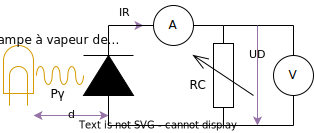
\includegraphics[width=12cm]{figures/montage.pdf}
    \caption{Diagramme électrique du montage expérimental \cite{notice} \cite{nicole}}
    \label{fig:montage}
\end{figure}

% \begin{itemize}
% \item Pas de liste du matériel!
% \item Décrire de manière succincte la méthode et l'appareillage utilisés. 
% \item Toutes les formules utilisées pour calculer les résultats doivent être énoncés clairement.
% \item Préciser les conditions expérimentales: toutes les valeurs utilisées pour le calcul doivent être mentionnées at leur valeurs fournies.
% \item Dans un article scientifique, toute la théorie et la description de la démarche expérimentale pour toutes les méthodes précèdent tous les résultats, puis une discussion donne la synthèse.
% \item Citer les schémas si repris (aussi si vous utilisez les illustrations faites par vos collègues).
% \end{itemize}
